\section{Ergebnisse}

\subsection{Bindungslänge}
\begin{frame}
\frametitle{Bindungslänge}
\begin{figure}[]
	\centering
	\begin{subfigure}{0.35\textwidth}
	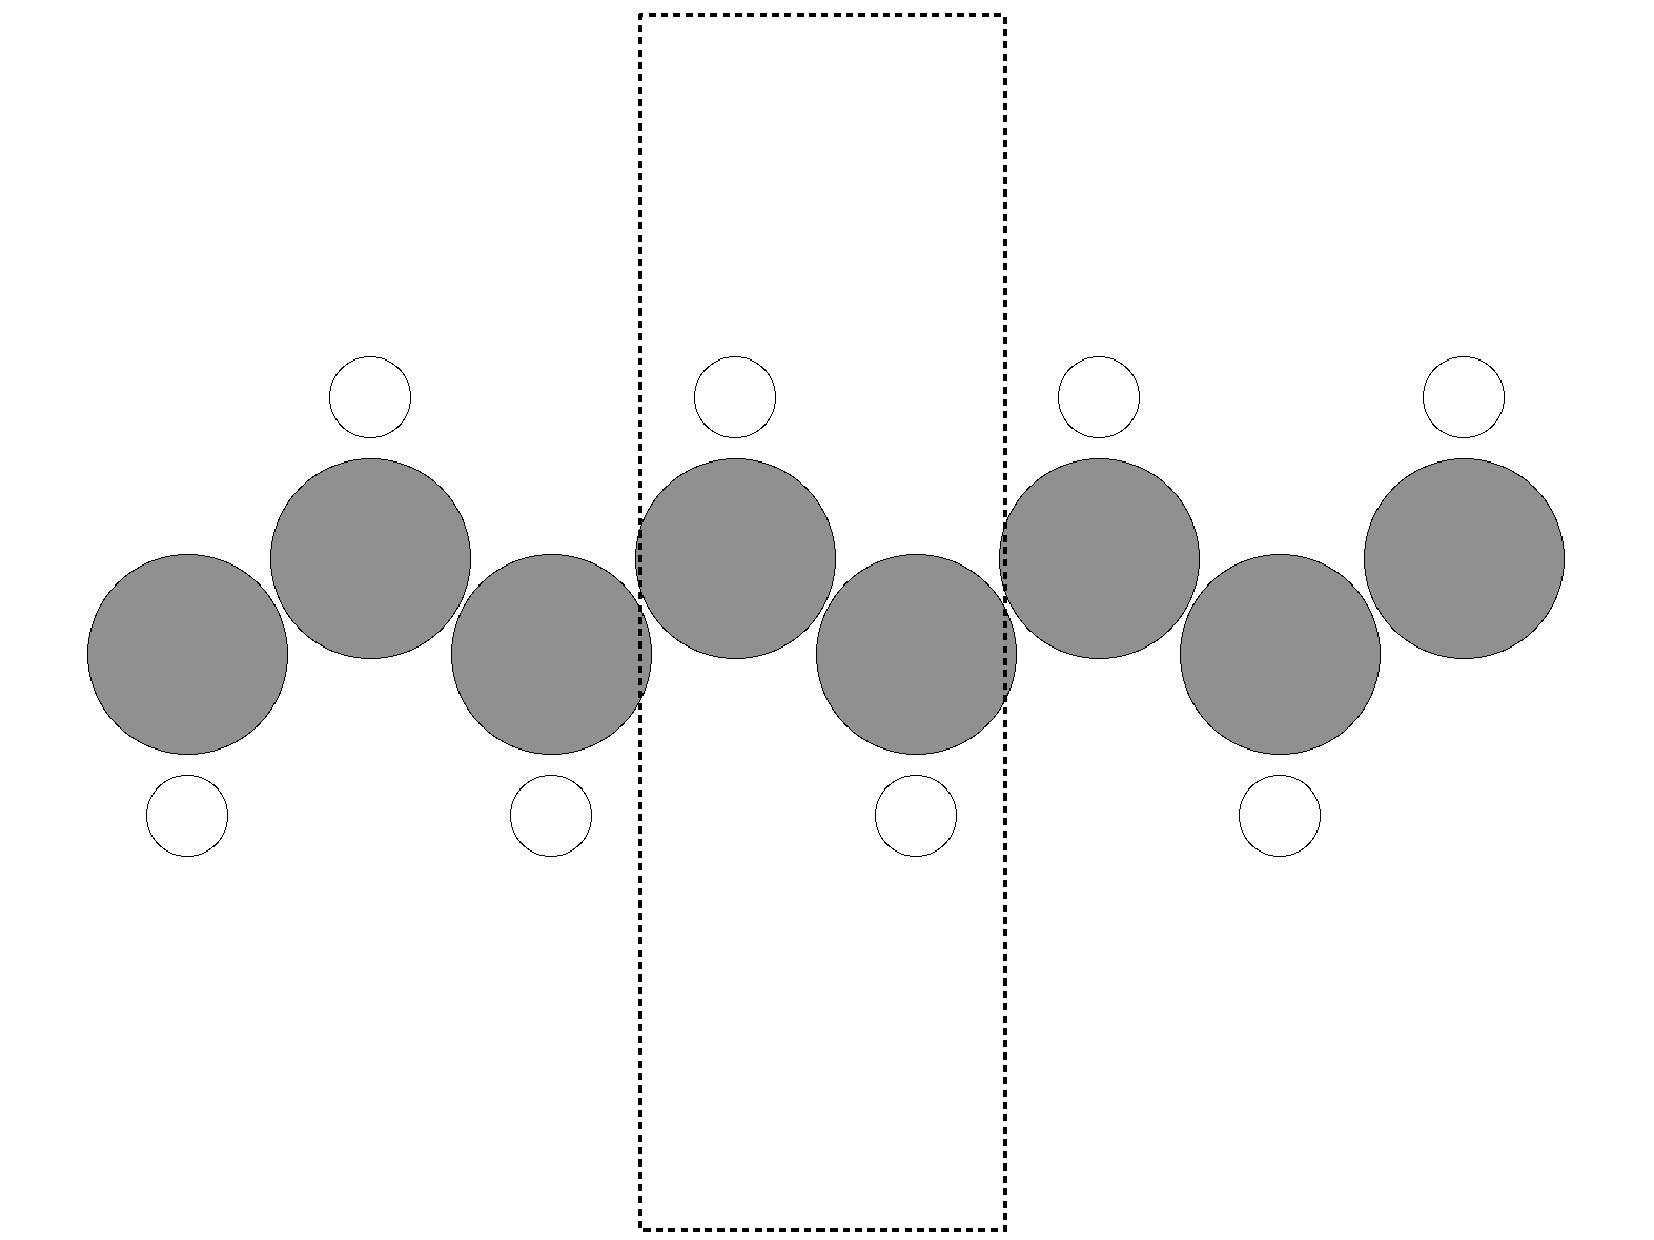
\includegraphics[width = \textwidth]{Images/polyacetylene/convergence/polyacetylene_nice_unit_cell}
	\caption{Schema: Einheitszelle \emph{trans}-Polyacetylen}
	\end{subfigure}\hspace*{1cm}
	\begin{subfigure}{0.45\textwidth}
		\centering
		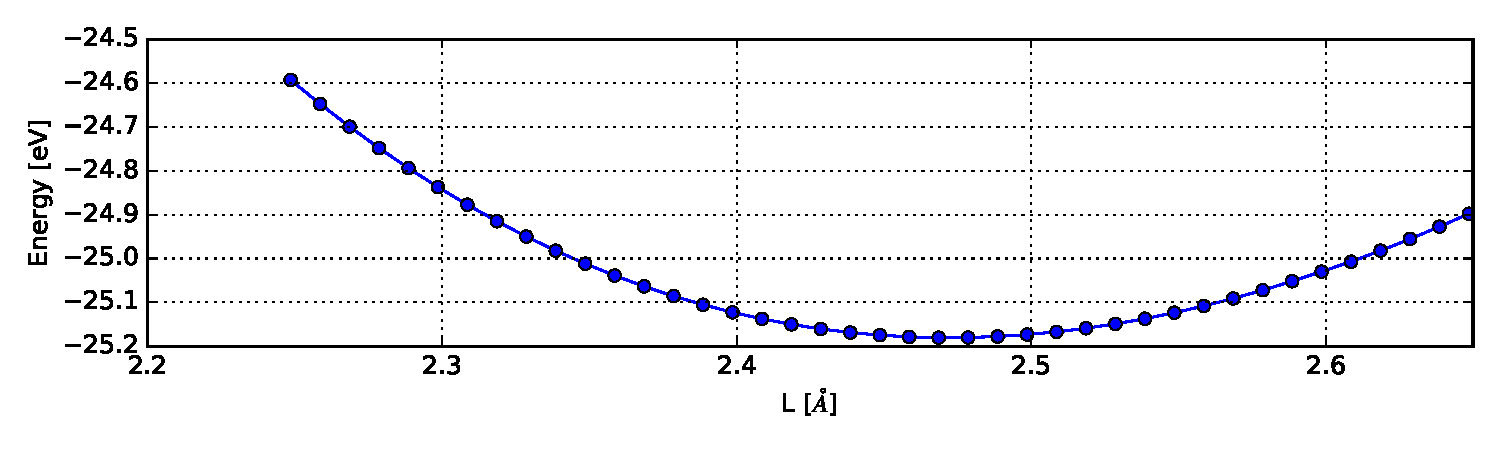
\includegraphics[width = \textwidth]{Images/polyacetylene/convergence/unit_cell_length}
		\caption{Grundzustandsenergie in Abhängigkeit von der Einheitszellenlänge}
		\label{image_poly_cell_len}
	\end{subfigure}
\end{figure}
\vspace*{-.5cm}

Berechnet: $a = \unit[1.23]{\AA}$\hfill Literaturwert: $a = \unit[1.2]{\AA}$
\end{frame}

\subsection{Verschiebung}
\begin{frame}
\frametitle{Verschiebung}
\begin{figure}
	\centering
	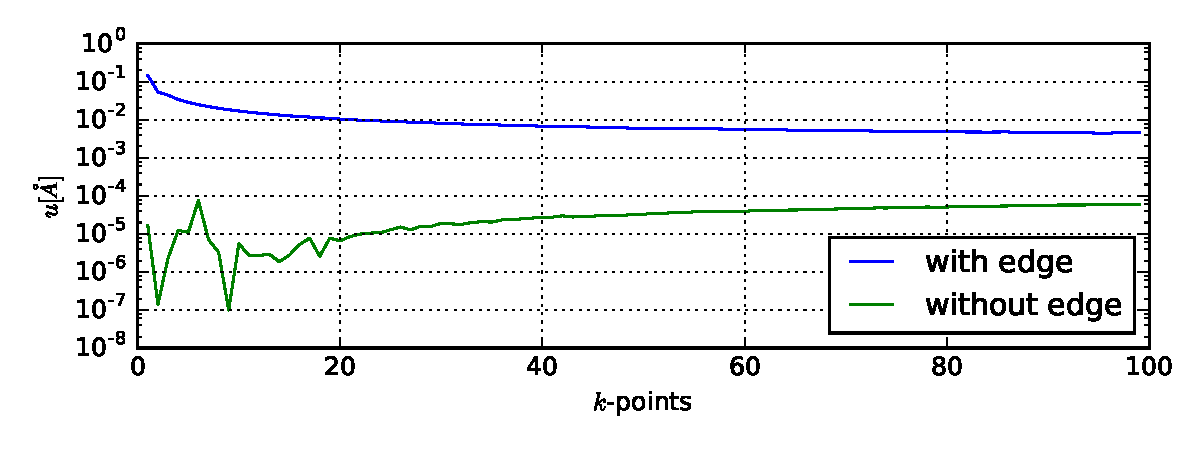
\includegraphics[width = \textwidth]{Images/polyacetylene/convergence/polyacetylene_displacement}
	\caption{Verschiebung $u$ in Abhängigkeit von den $k$-Punkten}
	\label{image_k_point_sampling_assymetry}
\end{figure}
\centering
\begin{tabular}{ll}
Ohne \textsc{Brillouin}-Zonen-Rand:& $u < \unit[10^{-4}]{\AA}$\\
Mit \textsc{Brillouin}-Zonen-Rand:&$u = \unit[5\cdot10^{-3}]{\AA}$\\
Literaturwert:& $u = \unit[0.042]{\AA}$
\end{tabular}
\end{frame}

\begin{frame}
\begin{figure}
	\centering
	\begin{subfigure}{.85\textwidth}
	\centering
	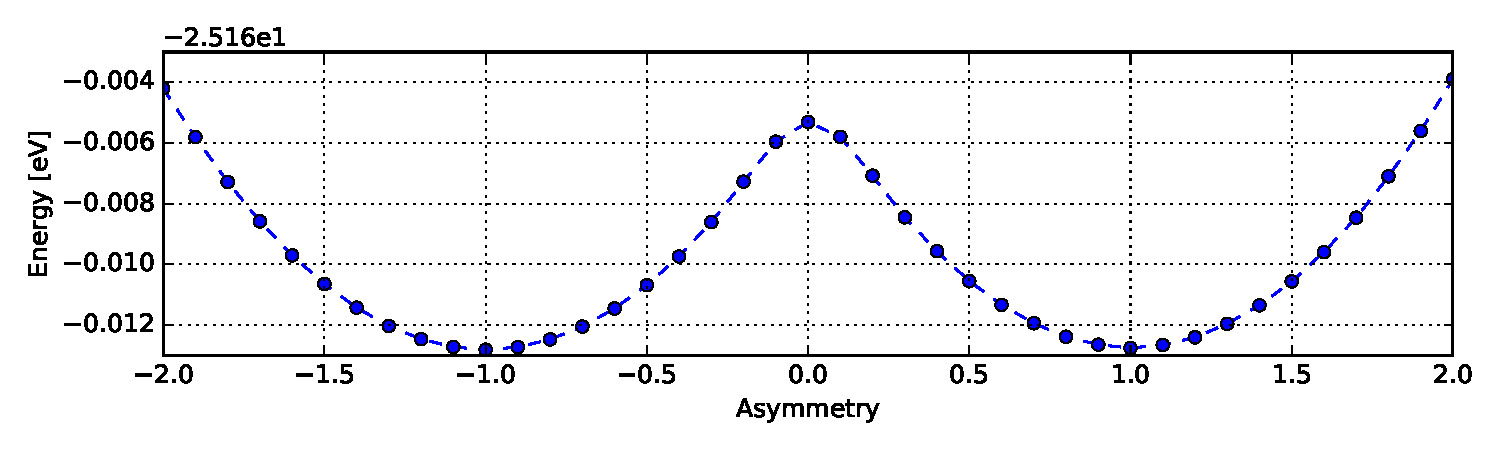
\includegraphics[width = \textwidth]{Images/polyacetylene/convergence/Potential_with_asymmetry}
	\caption{Mit $k$-Punkt am \textsc{Brillouin}-Zonen-Rand.}
	\label{image_potential_with_asymmetry}
	\end{subfigure}
	\begin{subfigure}{.85\textwidth}
	\centering
	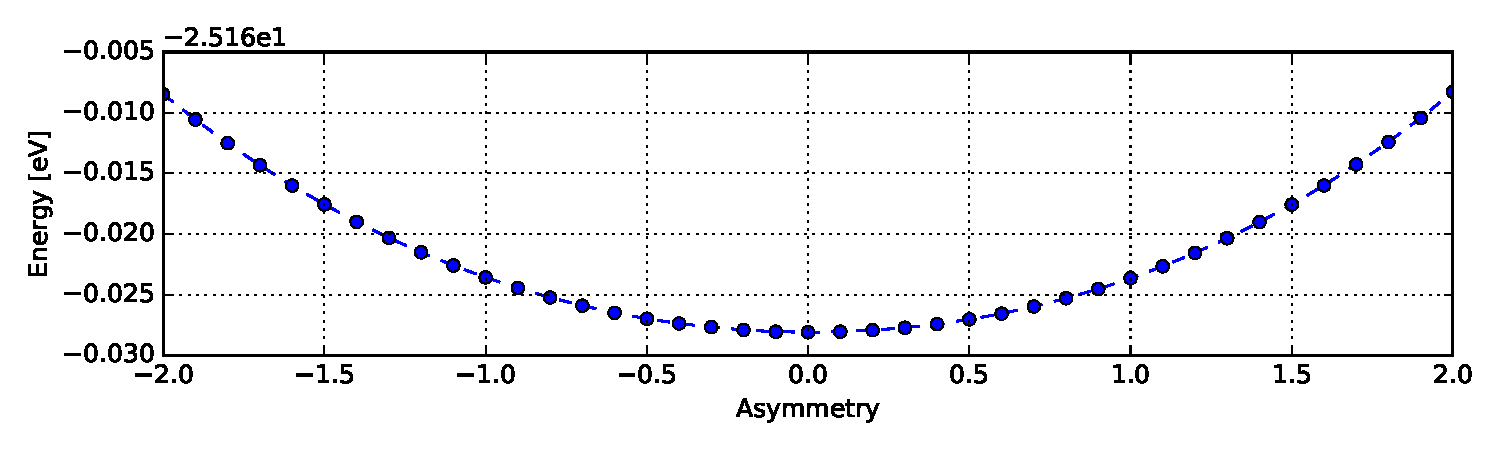
\includegraphics[width = \textwidth]{Images/polyacetylene/convergence/Potential_without_asymmetry}
	\caption{Ohne $k$-Punkt am \textsc{Brillouin}-Zonen-Rand.}
	\label{image_potential_without_asymmetry}
	\end{subfigure}
	\caption{Grundzustandsenergie in Abhängigkeit von der Asymmetrie $\nicefrac{u}{u_0}$.}
\end{figure}
\end{frame}

\begin{frame}
\begin{figure}
\centering
\begin{tikzpicture}[show background rectangle, scale = .65]
	\foreach \x in {0,...,7}{
		\draw[line width=1pt] (\x,0) .. controls (\x + 1, 2) and (\x - 1 , 2) .. cycle .. controls (\x + 1, -2) and (\x - 1 , -2) .. cycle;
	}
	\foreach \x in {0, 4}
	\foreach \y in {0, 1}
	\foreach \z in {-1, 1}
	\node at (\x + \y - \z + 1, \z) {\large +};
	\foreach \x in {0, 4}{
		\foreach \y in {0, 1}{
			\foreach \z in {-1, 1}{
				\node at (\x + \y - \z + 1, -\z) {\large -};
	}}}
	\draw[line width = 0.2] (-0.1, -1.8) -- +(-0.3, 0) -- +(-0.3 ,3.6) -- +(0,3.6);
	\draw[line width = 0.2] (1.1, -1.8) -- +(0.3, 0) -- +(0.3 ,3.6) -- +(0,3.6);
	\draw[line width = 0.2] (3.9, -1.8) -- +(-0.3, 0) -- +(-0.3 ,3.6) -- +(0,3.6);
	\draw[line width = 0.2] (7.1, -1.8) -- +(0.3, 0) -- +(0.3 ,3.6) -- +(0,3.6);
	\draw[dotted, line width = 1.5] (-0.6,0) -- (-1,0);
	\draw[dotted, line width = 1.5] (7.6,0) -- (8,0);
\end{tikzpicture}
\caption{Schema: p-Orbitale von alternierender $\pi$-Bindung.}
\end{figure}
\begin{figure}[]
	\centering
	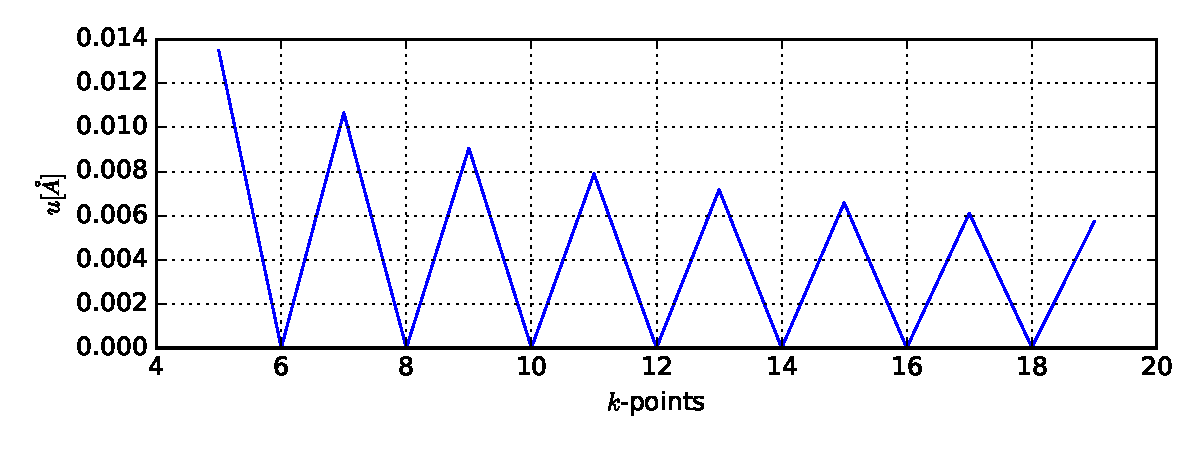
\includegraphics[width = .7\textwidth]{Images/polyacetylene/convergence/displacement_double_cell_poly}
	\caption{Verschiebung $u$ in Abhängigkeit von den $k$-Punkten für eine Einheitszelle mit vier CH-Gruppen.}
	\label{image_disp_double_cell_poly}
\end{figure}
\end{frame}

\begin{frame}
\begin{figure}
	\centering
	\begin{subfigure}{0.4\textwidth}
	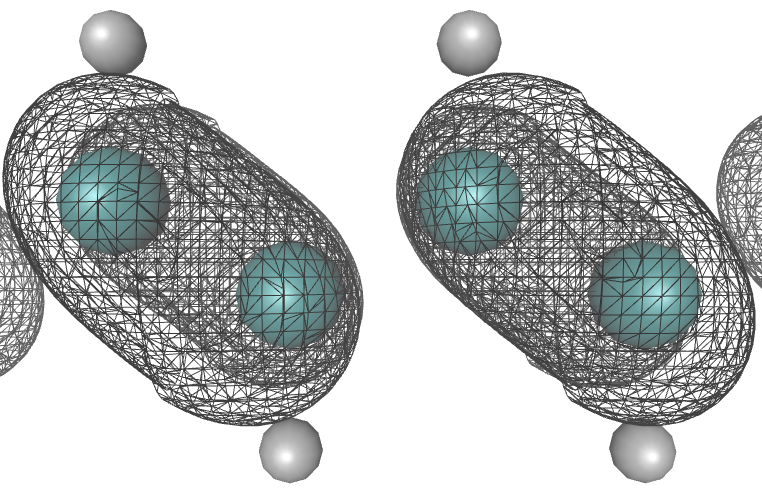
\includegraphics[width = \textwidth]{Images/polyacetylene/wavefunctions/Homo_Cut}
	\caption{HOMO-Band}
	\label{image_homo1}
	\end{subfigure}\hspace*{2cm}
	\begin{subfigure}{0.4\textwidth}
	\centering
	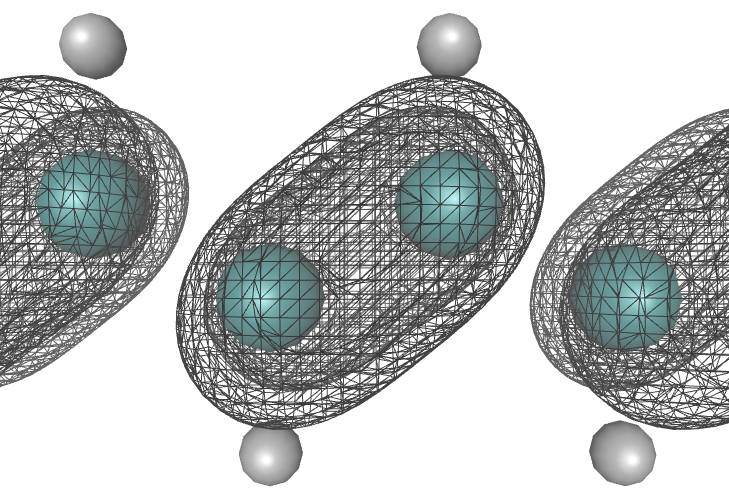
\includegraphics[width = \textwidth]{Images/polyacetylene/wavefunctions/LUMO_Cut}
	\caption{LUMO-Band}
	\label{image_lumo1}
	\end{subfigure}
	\begin{subfigure}{\textwidth}
	\centering
	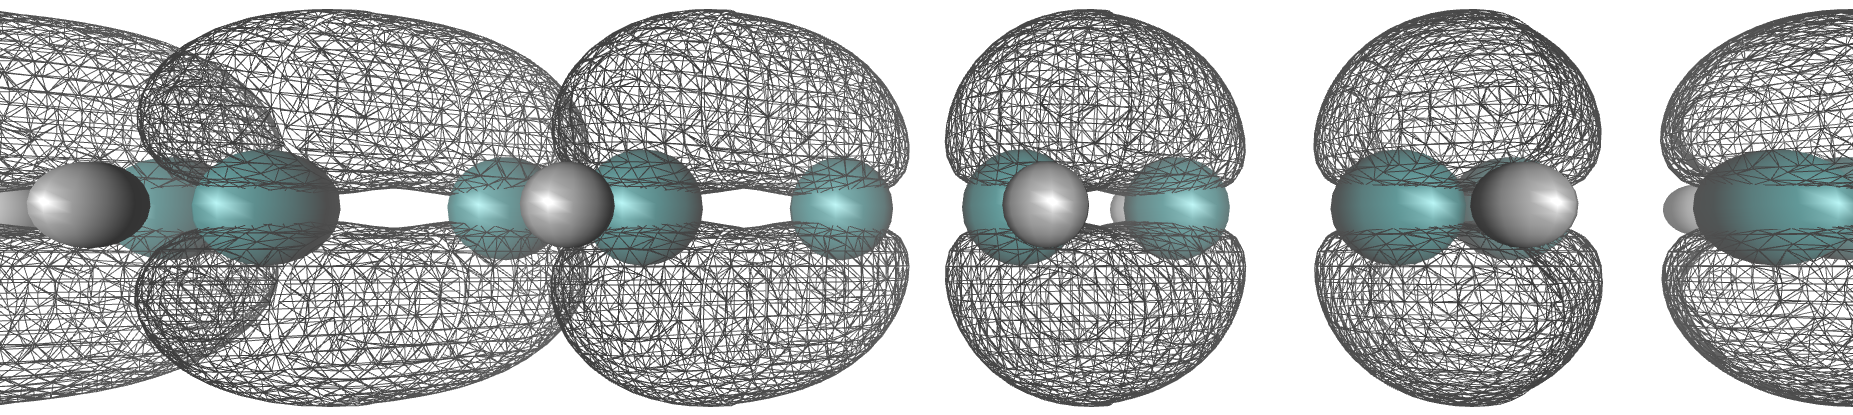
\includegraphics[width = 10cm]{Images/polyacetylene/wavefunctions/HOMO_Side_View}
	\caption{Seitenansicht HOMO-Band}
	\label{image_homo1_side_view}
	\end{subfigure}
	\caption{Isooberflächen für Zustände am \textsc{Brillouin}-Zonen-Rand.}
\end{figure}
\end{frame}

\subsection{Bandstruktur}
\begin{frame}
\frametitle{Bandstruktur}
\begin{minipage}{0.7\textwidth}
\begin{figure}
	\centering
	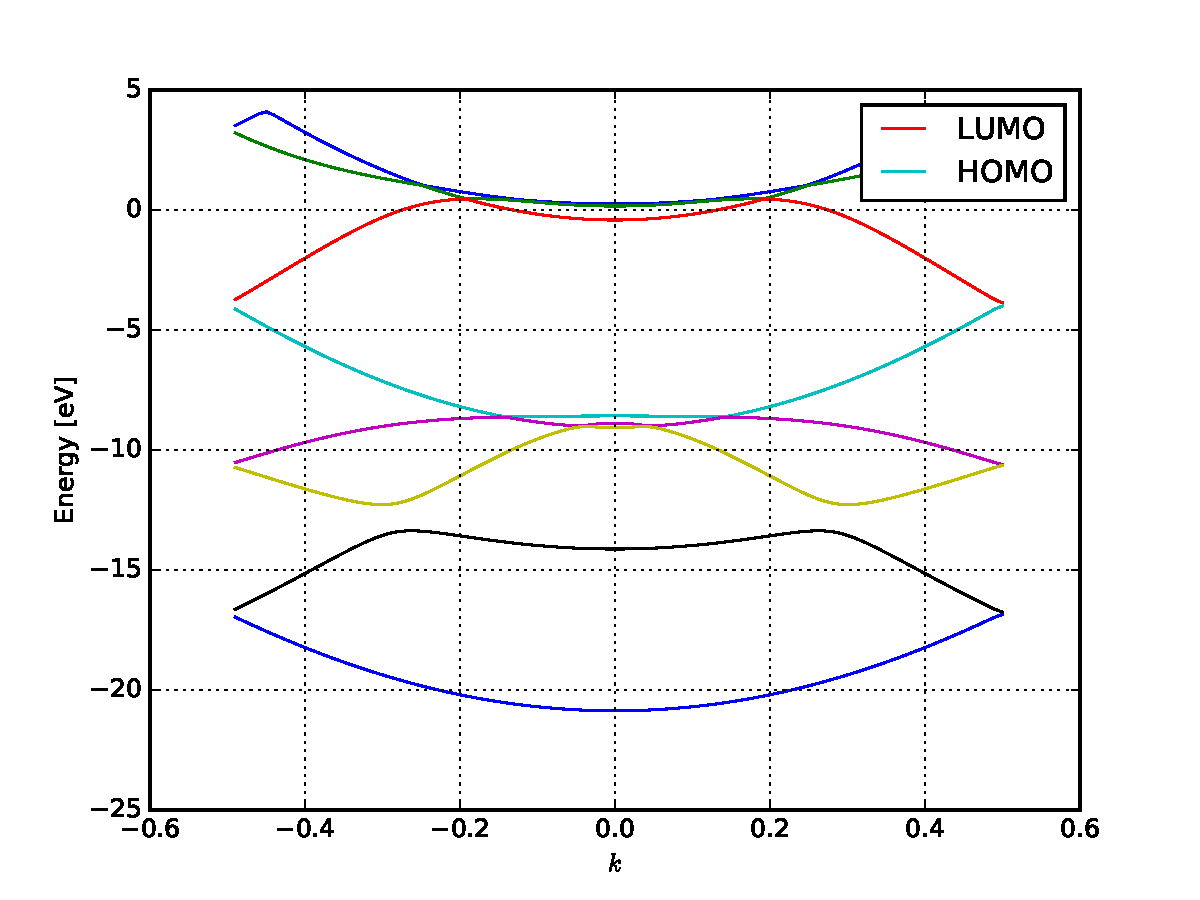
\includegraphics[width = \textwidth]{Images/polyacetylene/bands/band_structure}
	\caption{Bandstruktur \emph{trans}-Polyacetylen}
	\label{image_band_structure_relaxed_polyacetylene}
\end{figure}
\end{minipage}
\begin{minipage}{.29\textwidth}
\begin{itemize}
\setlength\itemsep{.2cm}
\item Berechnet:\\
$t_0 = \unit[2.62]{eV}$\\
Literaturwert:\\
$t_0 = \unit[2.5]{eV}$
\item Berechnet:\\
$\alpha = \unit[3.95]{eV/\AA}$\\
Literaturwert:\\
$\alpha = \unit[4.1]{eV/\AA}$
\item Berechnet:\\
$E_\text{Gap} = \unit[0.14]{eV}$\\
$\hspace*{1.15cm}(\unit[1.27]{eV})$\\
Literaturwert:\\
$E_\text{Gap} = \unit[1.4]{eV}$
\end{itemize}
\end{minipage}
\end{frame}

\begin{frame}
\frametitle{Kette von Wasserstoff-Atomen}
\begin{minipage}{0.6\textwidth}
Möglichst einfaches Testsystem für cDFT
\end{minipage}
\begin{minipage}{0.39\textwidth}
\centering
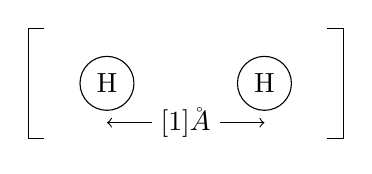
\begin{tikzpicture}
\node [circle, draw] at (0,0) {H};
\node [circle, draw] at (2,0) {H};
\draw (-0.8, 0.7) -- ++(-0.2, 0) -- ++(0, -1.4) -- ++(.2, 0);
\draw (2.8, 0.7) -- ++(0.2, 0) -- ++(0, -1.4) -- ++(-.2, 0);
\draw [<->] (0, -.5) -- +(2, 0) node [midway, fill = white] {$\small\unit[1]{\AA}$};
\end{tikzpicture}
\end{minipage}
\begin{figure}[]
	\centering
	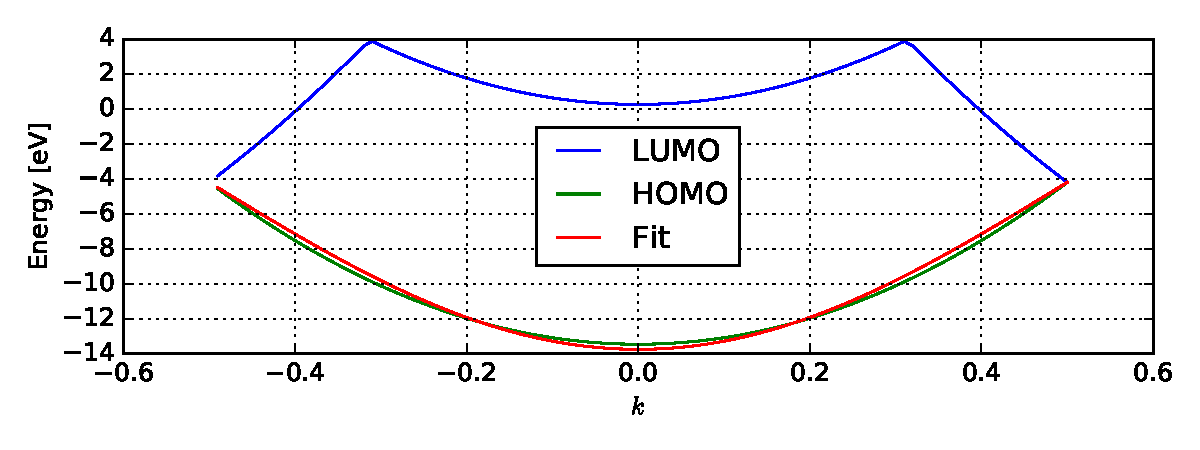
\includegraphics[width = 9cm]{Images/Hydrogen/bands/hydrogen_band_structure}
	\caption{Bandstruktur der Wasserstoff-Kette}
	\label{image_hydrogen_band_structure}
\end{figure}
\centering
$\Rightarrow\quad t_0 = \unit[4.8]{eV}$ 
\end{frame}

\subsection{Dichtefunktionaltheorie mit Zwangsbedingungen}
\begin{frame}{Dichtefunktionaltheorie mit Zwangsbedingungen (cDFT)}
\hspace*{-.5cm}
\begin{minipage}{0.75\textwidth}
	\vspace*{-1.5cm}
	\begin{itemize}
		\item Manuelles Verschieben von Ladung mittels externen Potentialen
		\item Definiere $i$ Regionen und Ladungen $N_i$
		\item Überlagerte Gauß-Kurven $w(\vec{r})$ zentriert an Kernpositionen $\vec{R}_j$
	\end{itemize}
\end{minipage}
\begin{minipage}{0.25\textwidth}
	\vspace*{-.8cm}
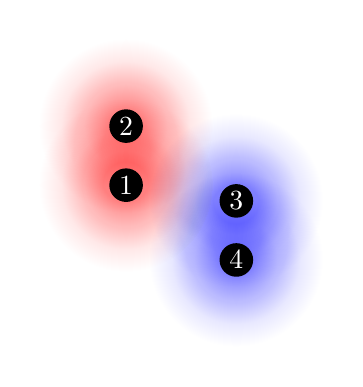
\begin{tikzpicture}[scale = 0.5]
	\foreach \i/\j/\color in {0/0.2/red, 0/1.7/red, 2.8/-0.2/blue, 2.8/-1.7/blue}{
		\foreach \r in {0, 0.01, ..., 1}{
			\fill[opacity = \r * 0.017, fill = \color] (\i, \j) circle ({2.5 * (1 - \r)});}}
	\foreach \i/\j/\num in {0/0.2/1, 0/1.7/2, 2.8/-0.2/3, 2.8/-1.7/4}{
		\node[fill = black, shape = circle, text = white, inner sep = 0.05cm] at (\i, \j)	 {\num};}
\end{tikzpicture}
\end{minipage}
\hspace*{-.5cm}
\begin{minipage}{\textwidth}
\vspace*{-1cm}
\begin{itemize}
	\item Minimierung der cDFT-Energie:
	\begin{align*}
	F\left[n\left(\vec{r}\right), U_i\right] &= E_0\left[n\left(\vec{r}\right)\right] + 
	\sum_i U_i\left(\int\dd\vec{r}\ w_i\left(\vec{r}\right)\ n\left(\vec{r}\right) - N_i\right)
	\end{align*}
	mit den Zwangsbedingungen:
	\begin{align*}
	0 &= \int\dd\vec{r}\ w_i\left(\vec{r}\right)\ n\left(\vec{r}\right) - N_i
	\end{align*}
\end{itemize}
\end{minipage}
\end{frame}

\subsection{Erstes Modell zur Beschreibung der Ladungsverschiebung}
\begin{frame}
\frametitle{Erstes Modell zur Beschreibung der Ladungsverschiebung}
\begin{itemize}
\item Hopping-Hamiltonian unverändert
\item Wellenfunktionen einheitlich variieren:
\begin{align*}
\Psi_k^{(v)}(q_\text{tb}) &= \sqrt{\frac{1}{2}-\frac{q_\text{tb}}{2}}c_k^{\dagger(e)}- \sqrt{\frac{1}{2}+\frac{q_\text{tb}}{2}}\frac{\epsilon_k - i \Delta_k}{|E_k|}c_{k}^{\dagger(o)}
\end{align*}
\item Grundzustandsenergie als Summe der Einteilchen-Energien:
\begin{align*}
E_0(q_\text{tb}) &= -\frac{4Nt_0}{\pi} \sqrt{1-q^2_\text{tb}}\\
&= -\frac{8t_0}{\pi} \sqrt{1 - \left(c\cdot q_\text{cDFT}\right)^2}
\end{align*}
\end{itemize}
\end{frame}

\begin{frame}
\frametitle{Standardabweichung der \textsc{Gauß}-Kurven}
\begin{itemize}
\item Zu kleines $\sigma\quad\Rightarrow\quad$ Lokalisiert Elektronen zu sehr
\item Zu großes $\sigma\quad\Rightarrow\quad$ Ungezielte Verschiebung
\item $\sigma$ mit leichtest möglicher Ladungsverschiebung
\end{itemize}
\begin{figure}[!t]
	\centering
	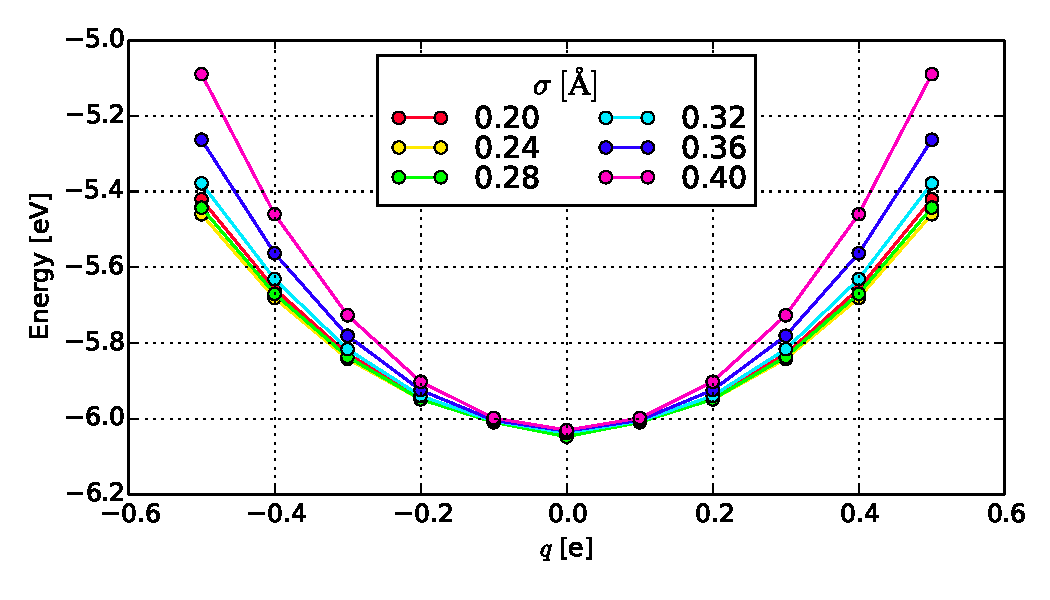
\includegraphics[width = 7.5cm]{Images/Hydrogen/charging/gaussian_sigmas}
	\caption{Grundzustandsenergie in Abhängigkeit von der verschobenen cDFT Ladung für verschiedene $\sigma$.}
	\label{image_gaussian_sigmas_hydrogen}
\end{figure}
\end{frame}

\begin{frame}
\frametitle{Berechnung des Hopping-Parameters}
\begin{minipage}{0.49\textwidth}
\begin{itemize}
\setlength{\itemsep}{.5cm}
\item Ergebnis: $t_0 = \unit[9.0]{eV}$
\item Referenzwert: $t_0 = \unit[4.8]{eV}$
\end{itemize}
\end{minipage}
\begin{minipage}{0.49\textwidth}
\begin{figure}
\centering
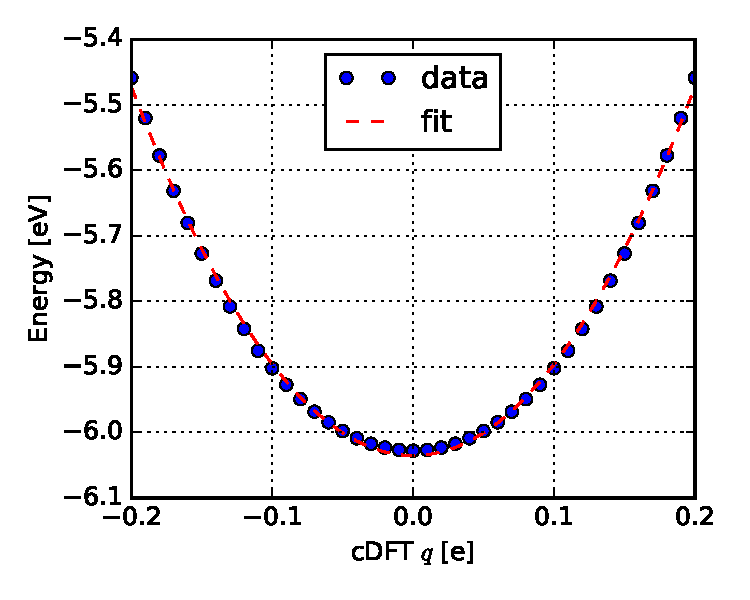
\includegraphics[width = \textwidth]{Images/Hydrogen/charging/energy_fit_normal_sigma}
\caption{Grundzustandsenergie in Abhängigkeit der verschobenen Ladung für $\sigma = \unit[0.24]{\AA}$}
\label{}
\end{figure}
\end{minipage}
\end{frame}

\begin{frame}
Ursachen:
\begin{itemize}
\item Grundzustandsenergie $\neq$ Summe Einteilchen-Energien
\item Zustände variieren nicht gleichmäßig
\end{itemize}
\begin{figure}
	\centering
	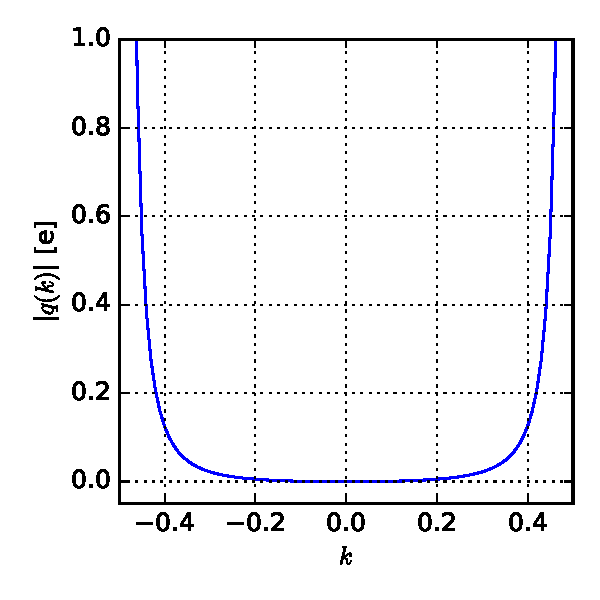
\includegraphics[width = 0.4\textwidth]{Images/Hydrogen/charging/charge_vs_k}
	\caption{Verschobene Ladung in Abhängigkeit von $k$ (tight-binding-Bild).}
	\label{image_tight_binding_q_vs_k}
\end{figure}
\end{frame}

\subsection{Zweites Modell zur Beschreibung der Ladungsverschiebung}
\begin{frame}
\frametitle{Zweites Modell zur Beschreibung der Ladungsverschiebung}
\begin{itemize}
\item Modifiziere Hopping-Hamiltonian:
\begin{align*}
\begin{pmatrix*}[c]
0 & \epsilon_k + i \Delta_k \\
\epsilon_k - i \Delta_k & 0
\end{pmatrix*} 
&\to 
\begin{pmatrix*}[c]
-V & \epsilon_k + i \Delta_k \\
\epsilon_k - i \Delta_k & V
\end{pmatrix*}
\end{align*}
\item Mit Eigenwerten:
\begin{align*}
E_k = \pm \sqrt{V^2+\epsilon_k^2+\Delta_k^2}
\end{align*}
\item Für Wasserstoff-Kette ($\Delta_k = 0$):
\begin{align*}
E_k &= \pm \sqrt{V^2 + \left(2t_0\cos(ka)\right)^2}
\end{align*}
\end{itemize}
\end{frame}

\begin{frame}
\begin{figure}
\centering
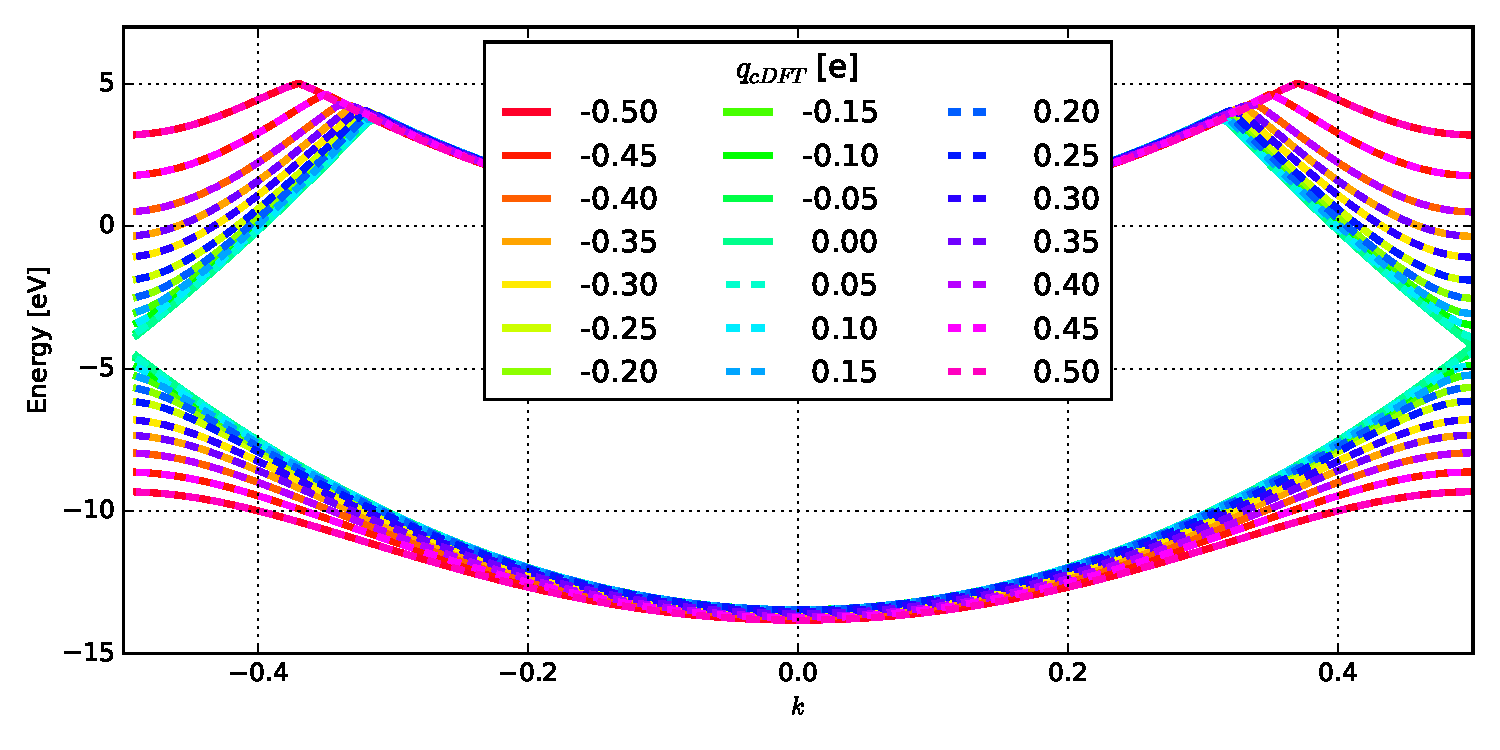
\includegraphics[width = 11cm]{Images/Hydrogen/charging/band_structure_q_1}
\caption{HOMO- and LUMO-Band für verschiedene Ladungsverschiebungen.}
\label{image_hydrogen_charged_bands}
\end{figure}
\begin{align*}
E_k &= \pm \sqrt{V^2 + \left(2t_0\cos(ka)\right)^2}
\end{align*}
\end{frame}

\begin{frame}
\begin{minipage}{0.49\textwidth}
\begin{itemize}
\item $V$ korrespondiert mit cDFT Potential-Stärken $U_i$
\item Erwartung von Hamiltonian:
\begin{align*}
U_1 = -U_2
\end{align*}
\item $V = c \cdot U$\\
$U = \frac{1}{2}(U_1 - U_2)$
\end{itemize}
\end{minipage}
\begin{minipage}{0.49\textwidth}
\begin{figure}
\centering
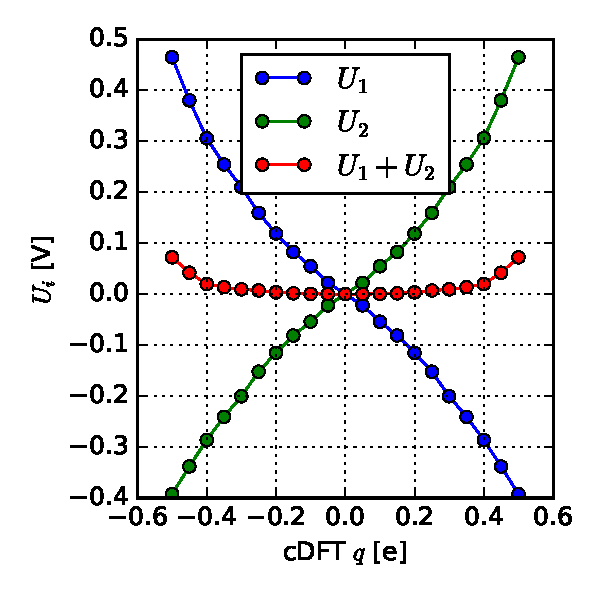
\includegraphics[width = \textwidth]{Images/Hydrogen/charging/potential_q_1}
\caption{cDFT potentials in respect to the displaced charge.\\}
\label{image_potentials_qs_1}
\end{figure}	
\end{minipage}
\end{frame}